%----------------------------------------------------------------------------
\chapter{Javaslat további funkciókra}\label{chapter:features}
%----------------------------------------------------------------------------
Diplomaterv feladatkiírásom része, hogy tegyek javaslatot olyan új modulokra vagy módosításokra, melyekkel a Jporta funkcionalitása bővíthető lenne.
A portál fejlesztése közben sok hasznos ötlet látott napvilágot.
Ebben a fejezetben az általam leghasznosabbnak ítélt két funkció indokoltságáról fogok beszélni, illetve vázolom egy lehetséges megvalósításhoz szükséges tervezési és implementációs lépéseket.

\section{Csapatrendszer}
Az első javaslatom egy csapatmunka támogatását lehetővé tevő funkció Jportába történő integrálása lenne.
A csapatrendszer feladata, hogy lehetővé tegye hallgatói csapatok kialakítását mind hallgatók, mind oktatók által, illetve a Jporta meglévő adminisztrációs funkcióit (értékelés, jelenlét, stb.) kiterjessze egyéni hallgatókról csapatokra.

A Jporta fejlesztésének megkezdésekor felmerült IIT-n használt egyéb, hasonló célú, oktatási rendszerek konszolidációja az új portálba, amivel a sok különböző alkalmazás működtetésére, karbantartására szánt idő és erőforrások csökkenthetőek lennének.
Az egyik ilyen rendszer a Hercules, melynek többek között a Szoftver projekt laboratórium -- régi nevén Szoftver labor 4. -- tárgy oktatásában van szerepe.
A tárgy keretében a hallgatók csapatban végzik el egy kisebb komplexitású szoftver tervezését, fejlesztését és dokumentálását.
A Hercules egyik legfontosabb funkciója is ehhez kapcsolódik, mégpedig hogy a félév elején biztosítja a hallgatók számára az említett csapatok kialakítását.
A jelenlegi rendszerben a hallgatóknak egy hét áll rendelkezésére a félév elején, hogy önállóan kialakítsák az 5-6 főből álló csapatokat, melyeket a Hercules felületén regisztrál a csapat vezetője.
A csapat regisztrációjakor meg kell adnia a csapat egyedi nevét, a csapattagok pedig a Neptun kódjukkal kerülnek azonosításra.
A határidő letelte után csapat nélkül marad hallgatókat a tárgy felelőse osztja be csapatokba saját belátása szerint. 

\subsection{Tervezés}
A tervezés első lépése a Hercules fent leírt funkciójának megismerése és az új rendszerhez való illesztési lehetőségeinek vizsgálata.
Ezután következhet csak egy új, csapatokat modellező osztály és a hozzá kapcsolódó üzleti logika megvalósítását segítő segédosztályok definiálása, továbbá a már meglévő kódrészek hozzáigazítása az új fejlesztéshez.

A csapatrendszerhez egyik alapvető funkciója a csapatok kialakítása.
A Hercules által implementált metódus kissé körülményes, kevés rugalmasságot biztosít a felhasználók számára.
Ezért az új rendszerben ennek a funkciónak némi átalakítással, modernizálással kell megvalósulni, igazodva a Jporta adottságaihoz, és kihasználva azokat.

A csapatalakítás menete az új rendszerben lehetne a következő:
\begin{enumerate}
    \item A hallgató belép a portálra és kiválasztja a tárgyat, amelyhez csapatot kíván alakítani.
    \item Kiválasztja az \textit{Új csapat alakítása} funkciót és megadja a csapat nevét.
    \item A létrejött csapatba meginvitálja hallgatótársait, amiről azok értesítést kapnak a Jporta beépített üzenetküldő rendszerén keresztül.
    \item A csapat meghívott tagjai eldöntik, hogy elfogadják-e a meghívást.
\end{enumerate}
Ebben az elgondolásban a csapatot létrehozó hallgató tölti be a csapatkapitány szerepét, ezért neki -- a csapatalakítás időszakában -- lehetősége van a csapatból csapattagok eltávolítására, illetve új csapattagok meghívására.
A csapatkapitány mindenképp részét képezi a csapatnak.
Minden hallgató tárgyanként legfeljebb egy csapatnak lehet tagja.
Azok a hallgatók, akik már tagjai egy csapatnak, de nem kapitányai csapatuknak, megszüntethetik tagságukat, és ezután van lehetőségük új csapathoz csatlakozni, vagy saját csapatot létrehozni.

A tárgy adatlapján az oktató megadhatja, hogy a tárgyban csapatmunka támogatására van-e szükség, és ha igen, akkor milyen alsó és felső korlát van a csapatok méretére, illetve mely időtartományban van lehetősége a hallgatóknak csapatot alakítani.
A tárgy oktatóinak bármikor lehetősége van új csapat létrehozására, illetve a meglévő csapatok törlésére, módosítására, de fontos, hogy ezzel a jogosultságukkal csak indokolt esetben éljenek.
Különös figyelmet kell fordítani a hallgatók csapatok közti mozgatására, mivel ez egy igen gyakori művelet, ami kitüntetett támogatás nélkül nehézkes és időigényes feladattá tud válni.

A csapatrendszer bevezetése miatt a portál megjelenésének és kezelésének is változnia kell.
Az oktatók egy tárgy adatlapján eddig az egyes hallgatókat értékelhették, adminisztrálhatták az órákon való részvételüket, adhattak ki nekik feladatot.
Az új rendszerben viszont, a csapatmunktát igénylő tárgyaknál ezeknek a funkcióknak csapatokon kell elvégezhetőeknek lenniük.

\subsection{Megvalósítás}
A csapatrendszer implementálásának alapja a csapatot megtestesítő Django modell létrehozása.
Ez az osztály írja le, milyen attribútumok tárolódnak az egyes csapatokról az adatbázisban, illetve hogy a Jporta rendszerének többi entitásával milyen kapcsolatban áll (lásd \ref{figure:teams-after}. ábra).
Ugyanez az osztály implementálja a csapatokhoz szorosan kapcsolódó üzleti logikát is.
Ahogy az a \ref{figure:teams-before}. és \ref{figure:teams-after}. ábra összehasonlításából jól látszik, a változtatások után a felhasználót reprezentáló \texttt{SwdUser} osztályt sok esetben a \texttt{Team} osztály váltja fel, ugyanakkor a tervezésnél már említettem, hogy a csapatok használata tárgyanként eltérő lehet, egy kapcsolótól függ csupán, melyet a tárgy oktatója választ meg.
Ezt a kettősséget úgy oldanám fel, hogy a háttérben mindkét esetben csapatokkal dolgozik a modell, ám ha az adott tárgy nem igényel csapatmunka-támogatást, akkor a rendszer minden felhasználó számára automatikusan létrehozza a felhasználó egyszemélyes csapatát.
A felhasználók számára ez egy teljesen transzparens folyamat, a megjelenítés a tárgyhoz beállítása alapján dönti el, hogy csapatok vagy egyéni felhasználók megjelenítésére van-e szükség egy adott esetben.

\begin{figure}[h]
    \centering
    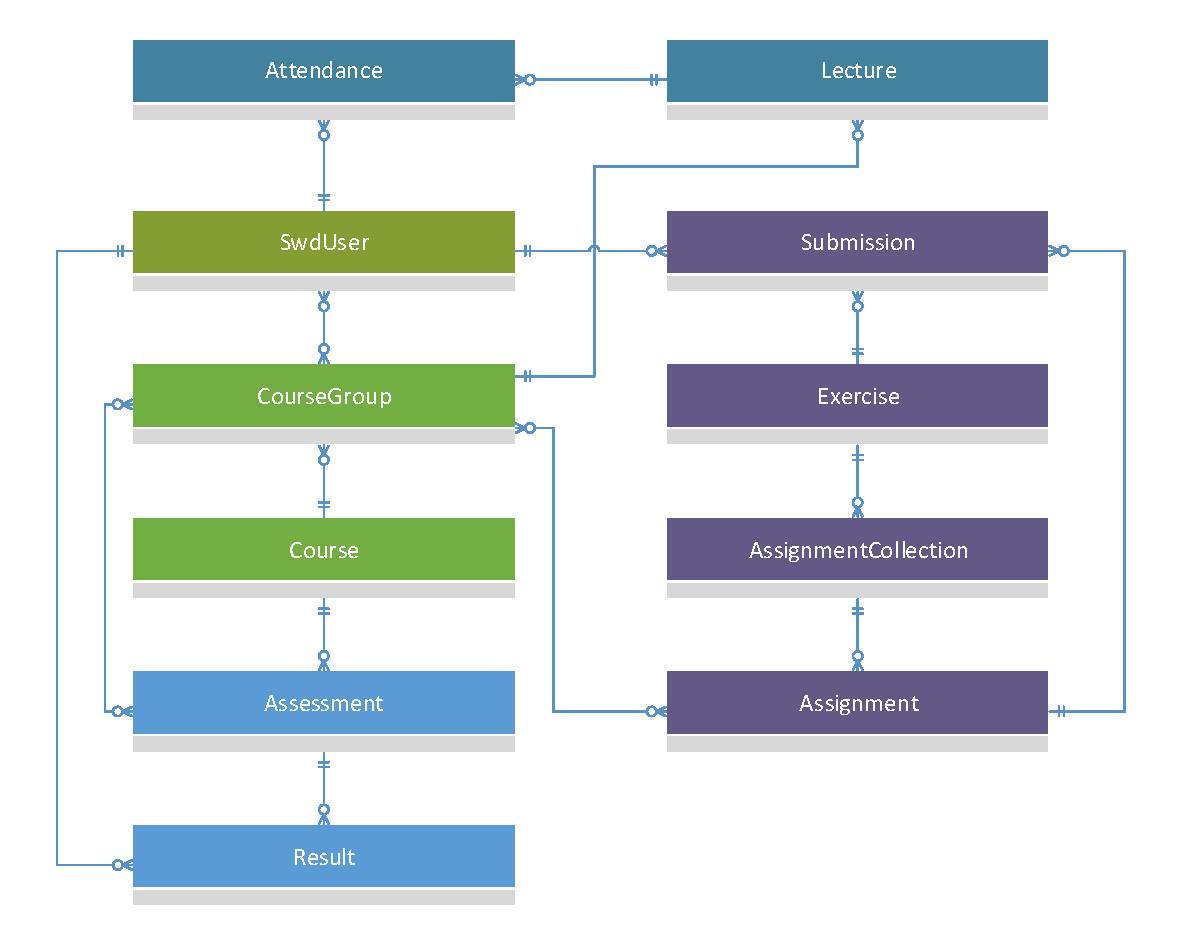
\includegraphics[width=\textwidth]{figures/teams-before}
    \caption{Jporta modellje csapatok nélkül}
    \label{figure:teams-before}
\end{figure}

\begin{figure}[h]
    \centering
    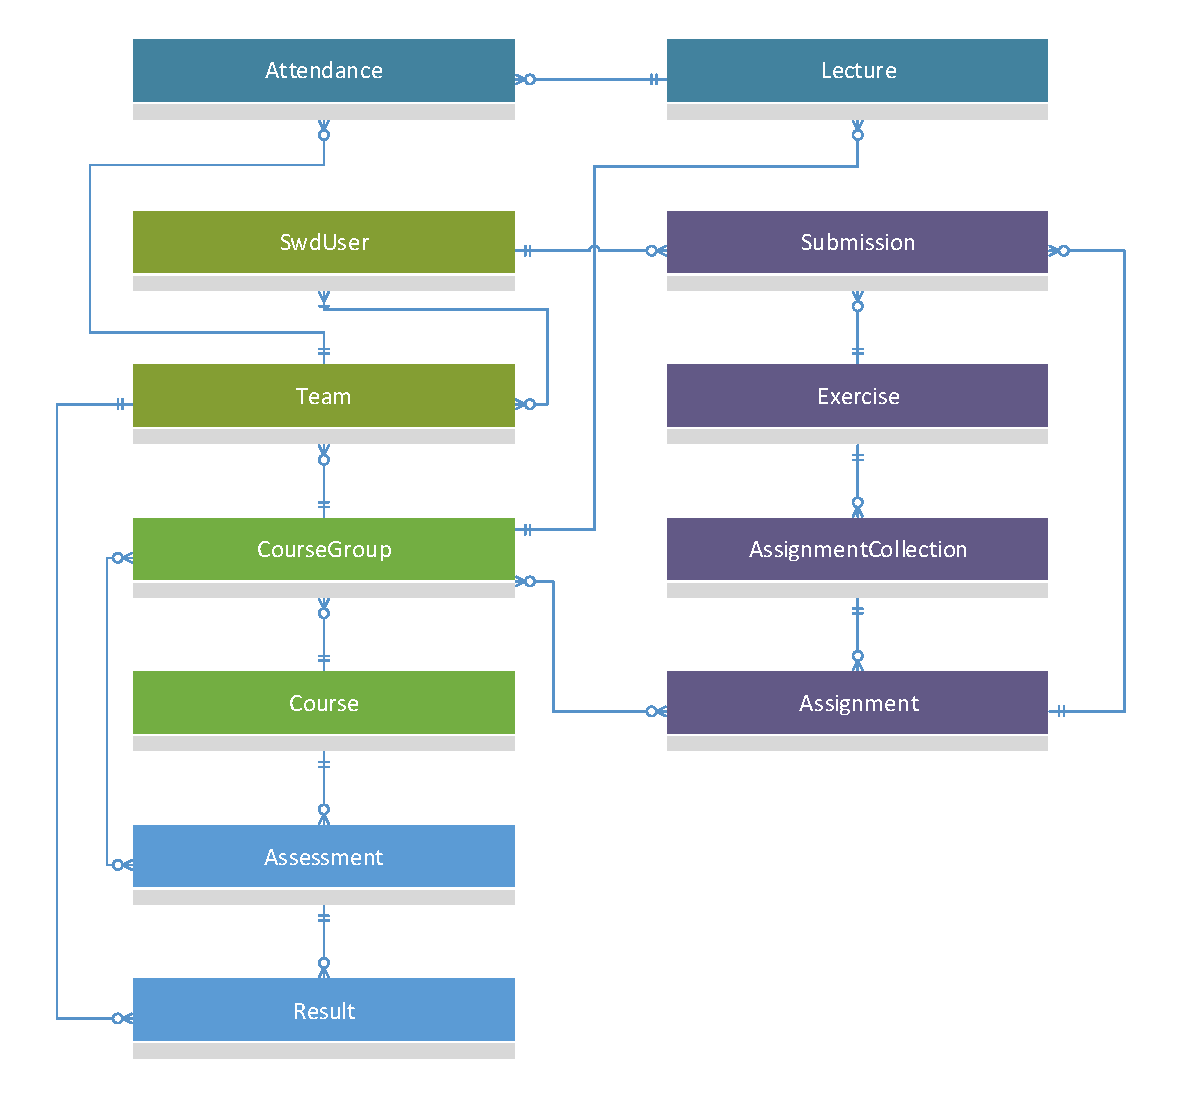
\includegraphics[width=\textwidth]{figures/teams-after}
    \caption{Jporta modellje csapatokkal}
    \label{figure:teams-after}
\end{figure}

További változás, hogy az eddig a kurzuscsoportok tagjainak nyilvántartására használt, Djangoba beépítetten érkező \texttt{Group} osztályt a fejlesztés során ki kell váltani egy több-több kapcsolatot nyilvántartó ``kapcsolótáblával'', mivel az egyes kurzuscsoportok (\texttt{CourseGroup}) most már nem felhasználóhoz (\texttt{SwdUser}), hanem csapatokhoz (\texttt{Team}) kapcsolódnak, ezeknek a tárolását viszont a \texttt{Group} osztály nem támogatja.

\section{Integráció verziókövető rendszerrel}
% verziókövető megismerésének hasznossága, DVCS, git
% működési elv, implementáció: pygit2, git-hook, repos vs. branches
TODO